\chapter{Relações}
Uma relação é um subconjunto de um produto cartesiano. Pode ser definida por uma lei ou pares ordenados escolhidos manualmente. É importante, quando iniciar os estudos sobre relações, fazer uso das representações gráficas como recurso visual para compreender o que está sendo enunciado. Outra observação importante é consolidar o conceito de um conjunto contínuo e conjunto discreto, com estas duas noções bem estabelecidas, ter-se-a mais confiança nas afirmações e respostas sobre relações.

\section{Representação de Relações}
Relações são subconjuntos de produtos cartesianos. Quando lidamos com relações entre conjuntos numéricos, temos um conjunto de pontos do plano cartesiano. Essa relação pode ser contida em quaisquer subconjuntos dos números reais. \par 
Para representar os pontos que pertencem a relação, utilizamos linhas sólidas, delimitando extremidades de segmentos com pontos fechados e regiões com áreas pintadas. Para representar pontos que não pertencem a relação, utilizamos linhas tracejadas, pontos abertos e regiões não-pintadas.

\begin{exemplo}
A relação $R \subseteq \mathbb{Z} \times \mathbb{R}, xRy \Leftrightarrow x^2 \ge y$ pode ser representada como no plano cartesiano abaixo.
\begin{figure}[H] 
\centering
	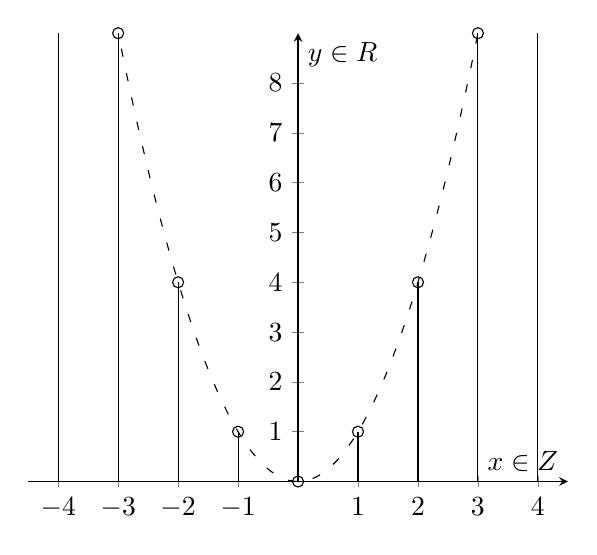
\begin{tikzpicture}
		\begin{axis}[
		axis lines = middle,
        xtick = {-4,-3,...,4},
        ytick = {0,1,...,8},
		xmin = -4.5,
        xmax = 4.5,
		ymin = 0,
        ymax = 9, 
        xlabel = $x \in \mathbb{Z}$,
        ylabel = $y \in \mathbb{R}$]
        \addplot[
        domain = -5:5,
        samples = 100,
        loosely dashed
        ]{x^2};
        \addplot+[ycomb, mark=o, black] plot coordinates
{(-4,16) (-3,9) (-2,4) (-1,1) (0,0) (1,1) (2,4) (3,9) (4,16)};
		\end{axis}
	\end{tikzpicture}
    \caption[Exemplo de Relação]{$R=\{(x,y) \in \mathbb{Z} \times \mathbb{R} \mid y<x^2\}$}
\end{figure}
\end{exemplo}

\section{Operações entre Relações}
Relações são conjuntos de pares ordenados e, portanto, podemos utilizar as operações de conjuntos entre relações. Para facilitar a visualização, essas operações também são representadas no plano cartesiano.


\begin{exemplo}

Dadas as relações $R \subseteq \mathbb{R}^2, xRy \Leftrightarrow x^2+y^2 < 4$  e $S \subseteq \mathbb{R}^2, xSy \Leftrightarrow y \ge x+2$, temos:

\begin{center}
\begin{tikzpicture}
    \begin{axis}[
        unit vector ratio* = 1 1 1,
        axis lines = middle,
        xtick = {-2,2},
        ytick = {-2,2},
		xmin = -3,
        width = 0.8\textwidth,
        height = 0.6\textwidth,
        xmax = 3,
		ymin = -3,
        ymax = 3, 
        xlabel = $x$,
        ylabel = $y$
      ]  
      \addplot[samples=100, domain=-2:2, dashed, name path=A] {sqrt(-x^2+4)}; 
      \addplot[samples=100, domain=-2:2, dashed, name path=B] {-sqrt(-x^2+4)}; 
      \path[name path=xaxis] (\pgfkeysvalueof{/pgfplots/xmin}, -3) -- (\pgfkeysvalueof{/pgfplots/xmax},3);
      \addplot[gray, color=lime!60!white] fill between[of=A and B, soft clip={domain=-3:3}];
  \end{axis}
  \end{tikzpicture}%
\quad \begin{tikzpicture}
    \begin{axis}[
        unit vector ratio* = 1 1 1,
        axis lines = middle,
        xtick = {-2},
        ytick = {2},
		xmin = -3,
        xmax = 3,
		ymin = -3,
        ymax = 3, 
        xlabel = $x$,
        ylabel = $y$,
        width = 0.8\textwidth,
        height = 0.6\textwidth,
      ]  
      \addplot[samples=100, domain=-3:2, name path=A] {x+2}; 
      \addplot[samples=100, domain=-3:1, color=olive!60!white,  name path=B] {3}; 
      \path[name path=xaxis] (\pgfkeysvalueof{/pgfplots/xmin}, -3) -- (\pgfkeysvalueof{/pgfplots/xmax},3);
      \addplot[gray, color=olive!60!white] fill between[of=A and B, soft clip={domain=-3:3}];
  \end{axis}
  \end{tikzpicture} \\
  \end{center}
  E abaixo podemos visualizar algumas operações entre as relações.
  \begin{center}
  \begin{tikzpicture}
    \begin{axis}[
        unit vector ratio* = 1 1 1,
        axis lines = middle,
        xtick = {-2,2},
        ytick = {-2,2},
		xmin = -3,
        xmax = 3,
		ymin = -3,
        ymax = 3, 
        xlabel = $x$,
        ylabel = $y$,
        width = 0.8\textwidth,
        height = 0.6\textwidth,
      ]  
     \addplot[samples=100, domain=-2:2, color=olive!60!white, name path=A] {sqrt(-x^2+4)}; 
      \addplot[samples=100, domain=-2:2, color=lime, name path=B] {-sqrt(-x^2+4)}; 
       \addplot[samples=100, domain=-3:3,  name path=C] {x+2};
        \addplot[samples=100, domain=-3:1, color=white, name path=D] {3};
        \addplot[samples=100, domain=0:3, dashed, name path=E] {sqrt(-x^2+4)}; 
      \addplot[samples=100, domain=-3:3, dashed, name path=F] {-sqrt(-x^2+4)}; 
      \path[name path=xaxis] (\pgfkeysvalueof{/pgfplots/xmin}, -3) -- (\pgfkeysvalueof{/pgfplots/xmax},3);
      \addplot[gray, color=lime!60!white] fill between[of=A and B, soft clip={domain=-3:3}];
   \addplot[gray, color=olive!60!white] fill between[of=C and D, soft clip={domain=-3:3}];
  \end{axis}
  \end{tikzpicture}%
  \begin{tikzpicture}
    \begin{axis}[
        unit vector ratio* = 1 1 1,
		width = 0.8\textwidth,
        height = 0.6\textwidth,
        axis lines = middle,
        xtick = {-2,2},
        ytick = {-2,2},
		xmin = -3,
        xmax = 3,
		ymin = -3,
        ymax = 3, 
        xlabel = $x$,
        ylabel = $y$
      ]  
      \addplot[samples=100, domain=-2:0, dashed, name path=A] {sqrt(-x^2+4)}; 
       \addplot[samples=100, domain=-3:4, thin, dashed, name path=E] {x+2};
       \addplot[samples=100, domain=-2:0, name path=B] {x+2}; 
         \addplot[samples=100, domain=0:2, dashed, name path=C] {sqrt(-x^2+4)}; 
      \addplot[samples=100, domain=-2:2, dashed, name path=D] {-sqrt(-x^2+4)}; 
      \path[name path=xaxis] (\pgfkeysvalueof{/pgfplots/xmin}, -3) -- (\pgfkeysvalueof{/pgfplots/xmax},3);
      \addplot[gray, color=lime!60!white] fill between[of=A and B, soft clip={domain=-3:3}];
  \end{axis}
  \end{tikzpicture} \\
   \begin{tikzpicture}
    \begin{axis}[
        unit vector ratio* = 1 1 1,
        axis lines = middle,
        width = 0.8\textwidth,
        height = 0.6\textwidth,
        xtick = {-2,2},
        ytick = {-2,2},
		xmin = -3,
        xmax = 3,
		ymin = -3,
        ymax = 3, 
        xlabel = $x$,
        ylabel = $y$
      ]  
      \addplot[samples=100, domain= -5:0, white, name path=A] {sqrt(-x^2+4)};
       \addplot[samples=100, domain=-2:0, dashed, name path=B] {x+2}; 
         \addplot[samples=100, domain=-5:5, dashed, name path=C] {sqrt(-x^2+4)}; 
      \addplot[samples=100, domain=-5:5, dashed, name path=D] {-sqrt(-x^2+4)}; 
      \path[name path=xaxis] (\pgfkeysvalueof{/pgfplots/xmin}, -3) -- (\pgfkeysvalueof{/pgfplots/xmax},3);
      \addplot[gray, color=lime!60!white] fill between[of=C and D, soft clip={domain=-3:3}];
       \addplot[gray, color=white] fill between[of=B and A, soft clip={domain=-3:3}];
  \end{axis}
  \end{tikzpicture}%
  \begin{tikzpicture}
    \begin{axis}[
        unit vector ratio* = 1 1 1,
        axis lines = middle,
        xtick = {-2,2},
        ytick = {-2,2},
        width = 0.8\textwidth,
        height = 0.6\textwidth,
		xmin = -3,
        xmax = 3,
		ymin = -3,
        ymax = 3, 
        xlabel = $x$,
        ylabel = $y$
      ]  
      \addplot[samples=100, domain=-2:0,  name path=A] {sqrt(-x^2+4)};
      \addplot[samples=100, domain=-5:5, dashed, name path=A] {sqrt(-x^2+4)}; 
      \addplot[samples=100, domain=-5:5, dashed, name path=B] {-sqrt(-x^2+4)}; 
      \addplot[samples=100, domain=-5:5, dashed, name path=C] {x+2}; 
      \addplot[samples=100, domain=-5:-2, name path=C_1] {x+2}; 
      \addplot[samples=100, domain=0:5, name path=C_2] {x+2}; 
      \addplot[samples=100, domain=-5:1, color=lime!60!white,  name path=D] {3}; 
      \path[name path=xaxis] (\pgfkeysvalueof{/pgfplots/xmin}, -3) -- (\pgfkeysvalueof{/pgfplots/xmax},3);
      \addplot[gray, color=olive!60!white] fill between[of=C and D, soft clip={domain=-3:3}];
   \addplot[gray, white] fill between[of=A and B, soft clip={domain=-3:3}];
  \end{axis}
  \end{tikzpicture}
  \end{center}
É importante ressaltar o cuidado a ser tomado com as extremidades das relações, onde as linhas são tracejadas ou preenchidas.
\end{exemplo}


\section{Propriedades das Relações}
\begin{itemize}
	\item \textbf{Reflexiva}: uma relação é dita reflexiva quando todo elemento $x$ se relaciona consigo mesmo, ou seja, existe o par $(x,x)$ para qualquer $x$.
	\item \textbf{Irreflexiva}: uma relação é dita irreflexiva se nenhum $x$ se relaciona consigo mesmo, ou seja, não existe o par $(x,x)$ para qualquer $x$.
	\item \textbf{Simétrica}: uma relação é dita simétrica se para todo par $(x,y)$ da relação, existe o par $(y,x)$.
	\item \textbf{Anti-simétrica}: uma relação é dita anti-simétrica se para todo par $(x,y)$ da relação, o par $(y,x)$ existe apenas se $x=y$.
\item \textbf{Assimétrica}: uma relação é dita assimétrica se para todo par $(x,y)$ da relação, não existe o par $(y,x)$.
	\item \textbf{Transitividade}: uma relação é dita transitiva se para quaisquer pares $(x,y)$ e $(y,z)$ da relação existe o par $(x,z)$.
\end{itemize}

\section{Relações de Equivalência}
Relações são ditas de \emph{equivalência} quando apresentam a simetria, a transitividade e a reflexividade. Estas relações definem subconjuntos nos quais os elementos se relacionam apenas entre si. Esses subconjuntos, chamados classes de equivalência, geram uma partição do conjunto inicial.
\begin{exemplo}
A relação $R \subseteq \mathbb{Q} \times \mathbb{Q}$: \[R = \left\lbrace(\frac{a}{b},\frac{c}{d}) \in \mathbb{Q} \times \mathbb{Q} \: | \: ad=bc\right\rbrace\] gera uma partição em $\mathbb{Q}$, onde cada elemento da partição é uma classe de frações equivalentes.
\end{exemplo}

\section{Relações de Ordem}
Um conjunto de pessoas, assim como um conjunto qualquer, podem apresentar uma relação de ordem. Desta forma, não significa necessariamente que existe uma maior importância entre elementos, mas sim uma ordenação. É possível - por meio da observação, por exemplo - que exista uma certa ordem em um processo, um planejamento, uma empresa, ou entre números.\par 
Como estamos em um material matemático, uma relação de ordem em um conjunto, significa dizer que quando relacionando dois a dois, um sempre será maior ou igual ao outro.

\subsection{Ordem Parcial}
Uma relação de ordem é dita \emph{parcial} se existem elementos que não se relacionam (em qualquer ordem).
\[R \subset A \times A , \ \left(\exists x,y \in A \right)\left( (x,y), (y,x) \not \in R \right)\]

\paragraph*{Ampla}
Uma relação de ordem parcial ampla é aquela em que $x R x$, como na relação ``... maior ou igual a ...'', onde todo número é igual a ele mesmo e, portanto, é maior ou igual.
\begin{itemize}
\item \textbf{Transitividade}:``se $x\ge y$ e $y\ge z$, então $x\ge z$''
\item \textbf{Antissimetria}: ``se $x\ge y$ e $y \ge x$, então $y =x$''
\item \textbf{Reflexividade}: ``$x \ge x$''
\end{itemize}

\paragraph*{Estrita}
Uma relação de ordem parcial estrita é aquela em que $(x,x) \not \in R$, como na relação ``... maior do que ...'', onde nenhum número é maior do que ele mesmo.
Assim, pode ser definida a partir de três propriedades:
\begin{itemize}
\item \textbf{Transitividade}:``se $x>y$ e $y>z$, então $x>z$''
\item \textbf{Assimetria}: ``se $x>y$, $y\not > x$''
\item \textbf{Irreflexividade}: ``$x \not > x$''
\end{itemize}

\subsection{Ordem Total}
Uma relação de ordem é chamada de \emph{ordem total} quando quaisquer dois elementos se relacionam. 
\paragraph*{Ampla}
A relação é dita ampla quando existem apenas duas opções, como na relação ``... maior ou igual a ...''.
\[\forall x,y \in A \left( x \le y \vee y \le x \right)\]
Este tipo de relação apresenta a chamada \emph{dicotomia}, onde todos os elementos se encaixam em uma das duas opções.

\paragraph*{Estrita}
A relação é dita estrita quando existem duas opções, ou seja, quando $x=x \Rightarrow (x,x) \not \in R$ então temos três casos: 
\[\forall x,y \in A \left( x=y \vee x < y \vee y < x \right)\]
Este tipo de relação apresenta a chamada \emph{tricotomia}, onde todos os elementos se encaixam em uma das três opções.

\subsection{Ordem Densa}
Uma relação de ordem em um conjunto é dita \emph{densa} se para todos elementos $x,y \in A$ existe algum elemento $z$ entre $x$ e $y$.
\[\forall x,y \in A \left( x<y \Rightarrow \exists z \in A \left(x<z<y\right) \right)\] \par 
O conjunto dos números reais é o principal exemplo de conjunto com uma relação de ordem densa, pois para quaisquer elementos $x,y \in \mathbb{R}$ tais que $x < y$, existe $\frac{x+y}{2} \in \mathbb{R}$ tal que $x < \frac{x+y}{2} < y$.

\begin{figure}[H]
\centering
	\begin{subfigure}[b]{0.3\textwidth}
	\centering
		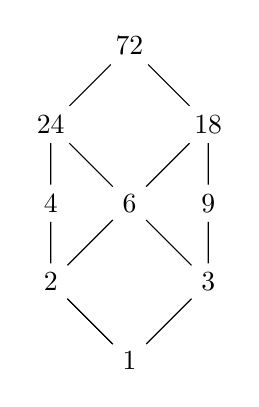
\begin{tikzpicture}
			\node (a) at (0,0) {$1$};
			\node (b) at (-1,1) {$2$};
			\node (c) at (1,1) {$3$};
			\node (d) at (0,2) {$6$};
			\node (e) at (1,2) {$9$};
			\node (f) at (-1,2) {$4$};
			\node (g) at (1,3) {$18$};
			\node (h) at (-1,3) {$24$};
			\node (i) at (0,4) {$72$};
			\draw (a) -- (b) -- (d) -- (g) -- (e) -- (c) -- (a);
			\draw (a) -- (b) -- (f) -- (h) -- (d) -- (c);
			\draw (h) -- (i) -- (g);
		\end{tikzpicture}
	\caption{Ordem Parcial}
	\end{subfigure}
	\quad
	\begin{subfigure}[b]{0.3\textwidth}
	\centering
		\begin{tikzpicture}
			\node (a) at (0,0) {$0$};
			\node (b) at (0,1) {$1$};
			\node (c) at (0,2) {$2$};
			\node (d) at (0,3) {$3$};
			\node (e) at (0,4) {$\vdots$};
			\draw (a) -- (b) -- (c) -- (d) -- (e);
		\end{tikzpicture}
	\caption{Ordem Total}
	\end{subfigure}
	\quad 
	\begin{subfigure}[b]{0.3\textwidth}
	\centering
		\begin{tikzpicture}
			\node (a) at (0,0) {$0$};
			\node (b) at (0,1) {$\vdots$};
			\node (c) at (0,2) {$1$};
			\node (d) at (0,3) {$\vdots$};
			\node (e) at (0,4) {$2$};
			\draw (a) -- (b) -- (c) -- (d) -- (e);
		\end{tikzpicture}
	\caption{Ordem Densa}
	\end{subfigure}
\caption{Diagramas de Hasse}
\end{figure}

\section{Funções}
\begin{df}
Sejam A e B dois conjuntos. Chamamos de \emph{função de $A$ em $B$} a uma relação que cada elemento de $A$ associa um único elemento de $B$, e denotamos simbolicamente por \begin{align*}
f: \ &A \rightarrow B \\
     &a \rightsquigarrow f(a)
\end{align*}
onde cada $a \in A$ está associado um único $b=f(a) \in B$. Chamamos $A$ de \emph{domínio da função $f$} e $B$ de \emph{contradomínio da função $f$}.
\end{df}
Uma função é uma relação entre dois conjuntos que relaciona um elemento de um conjunto (domínio) com um único do outro (contradomínio). Por definição, todo elemento do domínio precisa se relacionar com exatamente um elemento do contradomínio. O elemento do contradomínio correspondente ou do domínio é chamado de ``imagem'' ($\textrm{Im} \: f$). É importante saber que enquanto todo elemento do domínio precisa ter uma imagem, nem todo elemento do contradomínio precisa ter um correspondente do domínio.\par 

\begin{exemplo}
Seja a função $f$:\[f=\{(0,1),(2,5),(3,4),(5,8)\}\]
%imagem de funcao de um elipsoide pro outro
\end{exemplo}

Se $X \subset A$ e $f: A \rightarrow B$ denotamos por $f(X)$ ao conjunto $f(X)=\{f(x) : x \in X\} \subset B$ o qual chamamos de \textit{imagem de X pela f}. \par 
Se $f: A \rightarrow B$ é uma função e $y \in B$, denotamos por $f^{-1}(y)$ ao conjunto $f^{-1}(y)=\{x \in A : f(x)=y \}$ o qual chamamos de \emph{imagem inversa de $y$ pela $f$}. Se $y \not \in Im\:f$, $f^{-1}(y)= \emptyset$. \par 
Se $Y \subset B$ denotamos por $f^{-1}(Y)$ ao conjunto $f^{-1}(Y)=\{x\in A : f(x)=Y\}$ e chamamos tal conjunto de \emph{imagem inversa de $Y \subset B$ pela f}.

\subsection{Conjuntos}
\paragraph*{Domínio}
O \emph{domínio} de uma função, denotada como conjunto de partida, é o conjunto que contem todos os elementos de partida.
\paragraph*{Contradomínio}
O \emph{contradomínio} de uma função é o conjunto de chegada. O elemento parte do domínio e é associado a um do contradomínio.
\paragraph*{Imagem}
A \emph{imagem} de uma função é um conjunto contido no contradomínio cujos elementos são todos os elementos do contradomínio que são associados a um do domínio.\\
\begin{exemplo}
\begin{align*}
f: \ &\mathbb{N} \rightarrow \mathbb{R} \\
&x \rightsquigarrow x^2
\end{align*}
\end{exemplo}
Na nossa função f, nós temos como domínio $\mathbb{N}$ (conjunto de partida) e contradomínio $\mathbb{R}$ (conjunto de chegada). Nesse exemplo, podemos pegar um $x \in \mathbb{N}$, como 3, e seu elemento associado no contradomínio é o 9. O nosso conjunto $\textrm{Im} \, f$, portanto, é $\{0,1,4,9,16,25,\ldots\}$, que está contido em $\mathbb{R}$.

\subsection{Propriedades}
\paragraph{Injeção} Uma função é dita injetora quando: $\forall x,x'\in X, f(x)=f(x') \Rightarrow x=x'$. Ou seja, se dois elementos do domínio tem a mesma imagem, eles tem que ser o mesmo elemento. Isso nos diz que o conjunto $\textrm{Im} \,f$ tem o mesmo numero de elementos que nosso domínio.\\
\begin{exemplo}Seja a função $f$ definida por $f(x)=x^3$.\\
Vamos supor um x,x' tal que f(x)=f(x'). Para provarmos que a função é injetora, temos que provar que x=x'. Portanto:
\begin{align*}
&f(x)=f(x') &=\\
&(x)^3=(x')^3 &=\\
&\sqrt[3]{x^3}=\sqrt[3]{(x')^3}&=\\
&x=(x')
\end{align*}
\end{exemplo}

\paragraph{Sobrejeção} Uma função é sobrejetora quando $\forall y \in Y, \exists x \in X$ tal que $ y=f(x)$. Isso nos diz que todo y no contradomínio está contido na imagem, ou seja, $\textrm{Im} \, f$ e o contradomínio são iguais.\\
\begin{exemplo} Seja a função $f$ definida por $f(x)= x^3$. \par 
Queremos provar que todo y tem um x. Portanto:\\
\begin{align*}
&y=x^3 &=\\
&\sqrt[3]{y}=x
\end{align*}
Assim, temos que:
\begin{align*}
&f(\sqrt[3]{y}) &=\\
&(\sqrt[3]{y})^3 &= \\
&y
\end{align*}
\end{exemplo}

\paragraph{Bijeção} Uma função é bijetora quando ela satisfaz as condições de injeção e sobrejeção, ou seja, ela é sobrejetora e injetora. Como nos provamos nos últimos 2 seções que $f(x)=x^3$ é tanto injetora quanto sobrejetora, ela é uma função bijetora.\\
\begin{exemplo} Dada a função $f(x)= x+4$. 

%tabelinha de elipsoides que tem aqui: https://en.wikipedia.org/wiki/Bijection,_injection_and_surjection dai
\end{exemplo}

\subsection{Composição de Funções}
Se tivermos duas funções $f: A \rightarrow B$ e $g: B \rightarrow C$, uma função composta é denotada por: $f \circ g: A \rightarrow C$. $(f \circ g)(x)$ pode ser escrita em extenso como $f(g(x))$.\\
\begin{exemplo}
Se tivermos $f(x)=x+1$ e $g(x)=x^2$.\par 
$(f \circ g)(x)$ seria definida por:
\begin{align*}
&f(g(x)) &= \\
&f(x^2) &=\\
&x^2+1
\end{align*}
Enquanto $(g \circ f)(x)$ seria definida por:
\begin{align*}
&g(f(x)) &= \\
&g(x+1) &=\\
&(x+1)^2 &=\\
&x^2+2x+1
\end{align*}
\end{exemplo}
Com esse exemplo,podemos ver que a composição de funções não é comutativa.
%Elipsoides para mostrar comp. de funcoes. Aquela que tem 3 ovais e retas do 1 pro 2 pro 3. issae

\paragraph{Função Identidade} A função identidade, denominada por $\textrm{id}_x$, é uma função tal que $f \circ \textrm{id}_x=f$ e $\textrm{id}_x \circ f = f$. Essa função é $f(x)=x$.

\subsection{Função Inversa}
Uma função é \emph{inversível} se e somente se ela é bijetora. Ela leva um elemento do contradomínio para o domínio, e tem a propriedade $f^{-1}(f(x))=x$.
\begin{proof}
Suponhamos $f$ não-bijetora. Assim, $f$ não é injetora ou $f$ não é sobrejetora.\par 
Se $f$ não é injetora, existe $y \in CD f$ tal que $f^{-1}(y)={a,b} \subset D f$. Assim, existe $y \in D f^{-1}$ que possui duas imagens distintas e, portanto, $f^{-1}$ não é função.\par 
Se $f$ não é injetora, existe $y \in CD f$ tal que $f^{-1}(y)=\emptyset$. Assim, $f^{-1}$ possui um elemento de seu domínio que não possui imagem e, portanto, não é função.\par 
Logo, uma função é inversível se e somente se é bijetora.
\end{proof}

\section{Operações}
\begin{df}
Chamamos de \emph{operação (binária)} em um conjunto não vazio $A$ uma função
\begin{align*}
\mathcal{O}: A \times A &\rightarrow A \\
(a,b) &\rightsquigarrow \mathcal{O}(a,b)=a\mathcal{O}b
\end{align*}
A operação $\mathcal{O}$ é dita \emph{associativa} se $\forall a,b,c \in A$, tem-se $(a\mathcal{O}b)\mathcal{O}c=a\mathcal{O}(b\mathcal{O}c)$, e diz-se que é \emph{comutativa} se $\forall a,b \in A$, $a\mathcal{O}b=b\mathcal{O}a$.
\end{df}
